% stack-S-L-x.tex

% !TEX program = pdflatex
\documentclass[tikz]{standalone}
\usetikzlibrary{shapes.multipart, positioning}

\newcommand{\red}[1]{\textcolor{red}{#1}}
\newcommand{\blue}[1]{\textcolor{blue}{#1}}
\newcommand{\teal}[1]{\textcolor{teal}{#1}}

\begin{document}
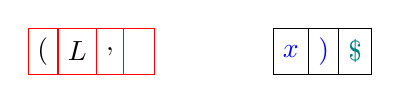
\begin{tikzpicture}[stack/.style = {rectangle split,
    rectangle split parts = #1, draw, anchor = center}]
  \node (stack) [stack = 4, draw = red, rectangle split horizontal] at (0,0)
    {$($\nodepart{two}$L$\nodepart{three}$,$\nodepart{four}};

  \node (input) [stack = 3, rectangle split horizontal, right = 1.5cm of stack]
  {\blue{$x$}\nodepart{two}\blue{$)$}\nodepart{three}\teal{\$}};
\end{tikzpicture}
\end{document}